\documentclass[12pt]{../notes}

\begin{document}
\ntitle{Handout 1.1: Introduction to Modern Regression Methods}

\section{About me}

\begin{figure}[H]
\centering
%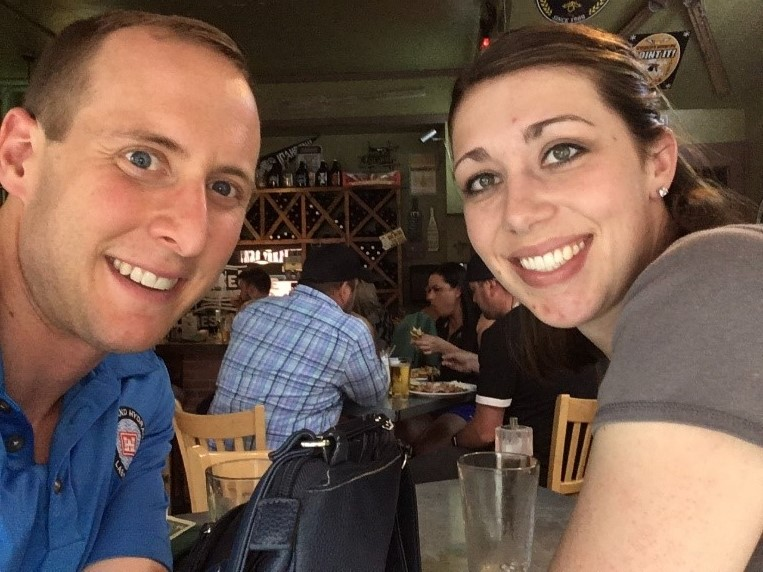
\includegraphics[width=0.59\textwidth]{../figures/module1/JessandBren2.jpg}
%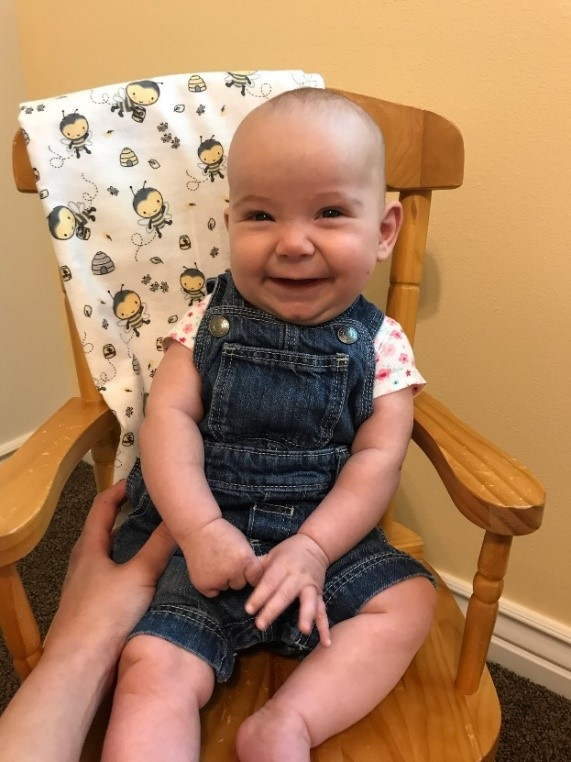
\includegraphics[width=0.39\textwidth]{../figures/module1/Lynnie.jpg}
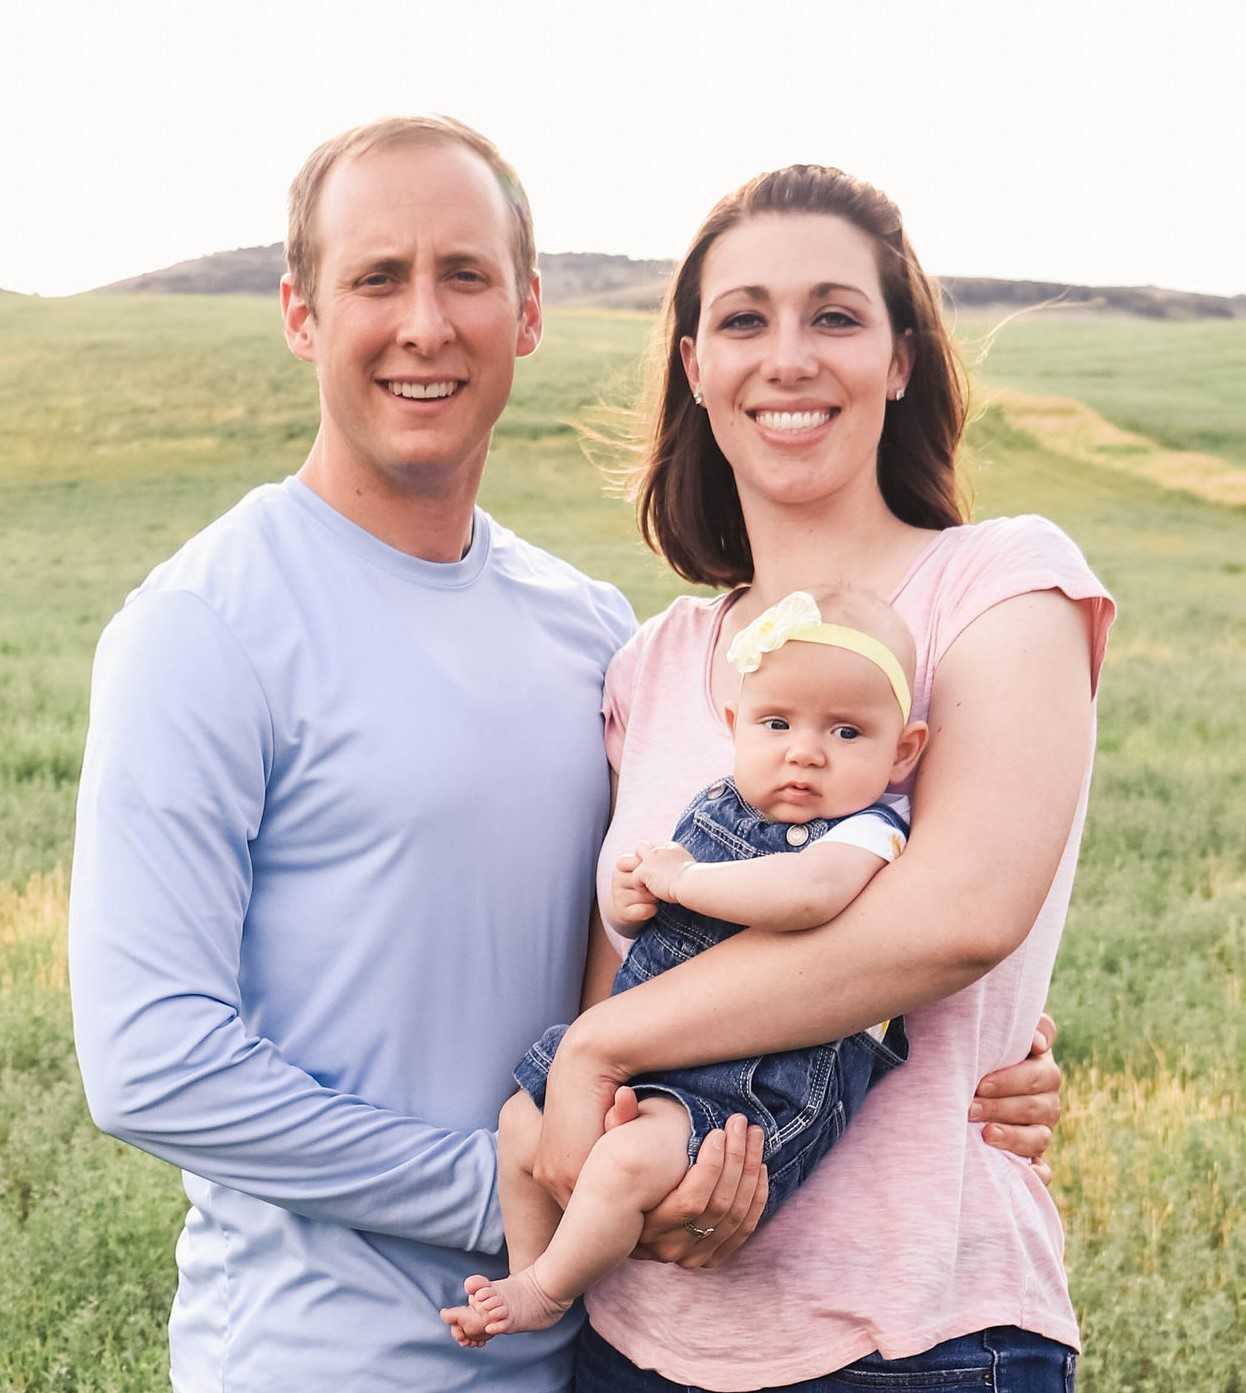
\includegraphics[width=0.5\textwidth]{../figures/module1/family.jpg}
\end{figure}

\begin{itemize}
\item Graduated from BYU-Idaho in 2014 with a Bachelors of Science in Applied Mathematics.
\item Graduated from Utah State University in 2019 with a PhD in Mathematical Sciences.
\item Current interests include basketball, cross country skiing, hiking and spending time with my wife and daughter.
\end{itemize}


\question{What is a creative, yet appropriate, question that you have about the life/career of the instructor?}

\begin{minipage}[l][2cm][c]{\textwidth}
%\begin{comment}

%\end{comment}
\end{minipage}

\section{Why Modern Regression Methods?}

Statistics, in the words of Dr. Bin Yu, is the ``science that solves data problems.'' This science becomes more and more relevant in a world inundated with data. From the late Leo Breiman:

\begin{quotation}
The uses of statistics pervade our society. They are used and terribly misused all through the social sciences and health fields. ... It is surprising how much the world around us depends on the use of statistics. ... It’s odd that even though the articles involving statistics in the newspapers far outnumber those involving say, physics or chemistry, people in general know very little about what we do.
\end{quotation}

In this class, we will learn several of the foundational approaches for using data to make \textbf{predictions}. Perhaps more importantly, we will discuss the \textbf{cautions} we must consider when using and interpreting model output. 

\question{Why are YOU taking this course?}

\begin{minipage}[l][3cm][c]{\textwidth}
%\begin{comment}

%\end{comment}
\end{minipage}


\section{Functional vs Statistical Modeling}

We learn about functions in Math 1050 (College Algebra), a functional model takes a set of inputs $X$ and produces a (set of) outputs $Y$, i.e.
\[Y = f(X)\]

Example: 
You write a function to model the profits from your lemonade stand. You rent the stand for \$200 a month and sell each glass of lemonade for \$1.00. If it costs you \$0.25 to make the lemonade then your monthly profits $Y$ could be modeled as a function of the number of lemonade glasses you sell $x$
\[Y = 0.75x - 200.\] 

The key to a functional model is that each input $x$ produces a \textbf{unique} output $Y$.

\vspace{0.5cm}
In a \textbf{statistical model} we assume that the values of $Y$ can be modeled by a function \textit{plus} some ``random noise'' $\epsilon$. The presence of the $\epsilon$ term allows for many different values of $Y$ for the same set in inputs $x$. 
\[Y = f(X) + \epsilon\]

Example: The relationship between ground snow and elevation in Utah (see figure \ref{fig:sampleScatter}). 

\begin{figure}[H]
\centering
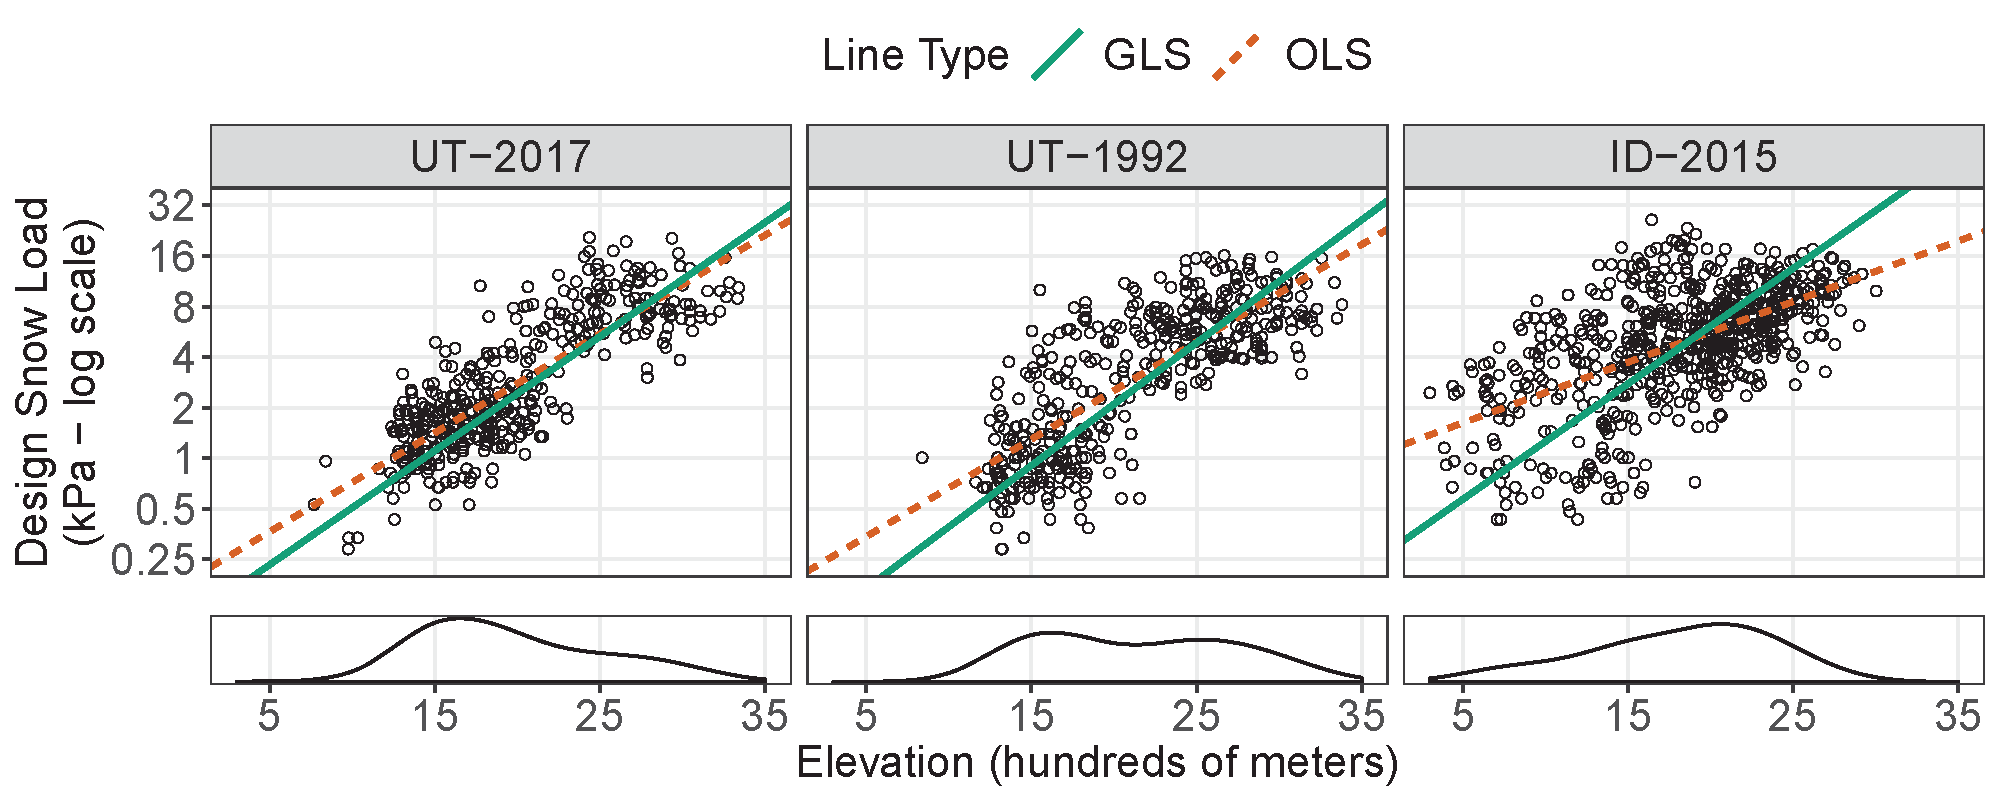
\includegraphics[width=0.8\textwidth]{../figures/module1/sampleScatter.png}
\caption{Plot of design ground snow loads (log-scale) vs elevation in and near Utah.}
\label{fig:sampleScatter}
\end{figure}

\section{The Key Assumption (why this class exists)}
\textbf{The key assumption} (and the foundation for this course) we make is that $\epsilon$ follows a probability distribution. Specifically we assume that 
\begin{equation}
\epsilon \sim^{i.i.d} N(0, \sigma^2).
\label{eq:resid}
\end{equation}
\textit{If this assumption is valid,} then our \textbf{estimates} of the \textbf{model parameters} will come from well-defined probability distributions, which will allow us to determine if the linear relationships between our explanatory variables and our response variable are significant. This process is often called \textbf{statistical inference}. 

\question{What do each of the symbols mean in (\ref{eq:resid}) and why might they be important?}

\begin{minipage}[l][5cm][c]{\textwidth}
%\begin{comment}
\note{
\begin{itemize}
\item \textbf{independence:} Knowing the value of one of the residuals should tell us nothing about the rest.
\item \textbf{identically distributed:} Each of the residuals come from the same probability distribution. 
\item \textbf{zero mean:} The residuals have an average value of zero (i.e. the model is not biased). 
\item \textbf{constant variance:} The spread of the residuals is constant across all predictions. 
\end{itemize}
}

\note{
Why they are important is something we will talk about for the next several weeks. 
}
%\end{comment}
\end{minipage}

\section{Why ``Linear Regression''?}
\subsection{Why Linear?}
Model are composed of:
\begin{itemize}
\item \textbf{coefficients:} These are \textit{constant} values that are \textit{estimated} to optimize the model fit. 
\item \textbf{variables:} These are the \textit{observed} values, calculated from the data that we use to estimate parameters or make predictions. 
\end{itemize}

A model is considered ``linear'' if it can be written as a sum of coefficients $\beta$ multiplied by a set of variables $x$, i.e. 
\[Y = \sum_i\beta_iX_i\]

This means that you can have nonlinear variables as long as the coefficients are linear.

\question{Which of the following models are linear and which are non-linear?
% First three are linear, last one is not. 
\begin{itemize}
\item $Y = \beta_0 + \beta_1X_1+\epsilon$
\item $Y = \beta_0 + \beta_1e^{X_1}+\epsilon$
\item $Y = \beta_0 + \beta_1X_1X_2+\epsilon$
\item $Y = \beta_0 + X_1^{\beta_1}+\epsilon$
\end{itemize}}

%\note{First three are linear, last one is not. }

\subsection{Why Regression?}
Based on concept that things tend to ``regress'' to the mean:

Example: heights of fathers vs sons:
\begin{itemize}
\item Tall fathers tend to have tall sons, but those sons will tend to be shorter than their fathers. 
\item Short fathers tend to have short sons, but those sons will tend to be taller than their fathers. 
\item Thus, a line comparing ``standard deviations'' of fathers and sons heights will have a slope approximately equal to one, while the \textbf{regression} line will have a slope that is less than one. 
\item Because things regress to the mean, the regression line will always be flatter than the standard deviation line. 
\end{itemize}

\begin{figure}[H]
\centering
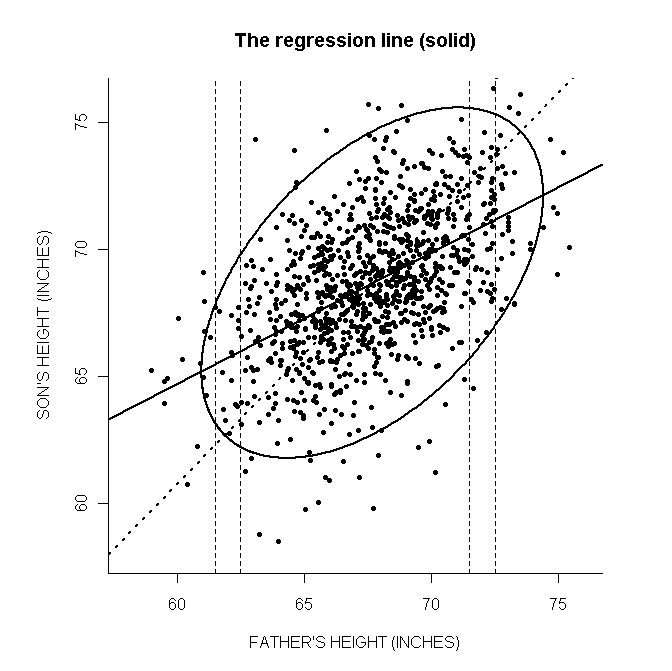
\includegraphics[width=0.5\textwidth]{../figures/module1/heightScatter.png}
\caption{Plot of father vs sons' heights. The dotted line is the standard deviation line while the solid line is the regression line.}
\end{figure}

























\end{document}